

\section{Circadian rhythms}
Every human being, and indeed many or most living things, contains at
least one internal clock (Ko and Takahashi,~2006; Partch et al.,~2014;
Rosato et al., 2006). Biological clocks with a period of 
approximately 24 hours are called \textit{circadian} clocks (meaning
``about a day''). The consequences of an incorrectly working clock
become obvious when one flies from Canada to Japan.

The circadian clock is a chemical limit cycle oscillator. Ronald
Konopka and Seymour Benzer~(1971), working in the fruit fly
\textit{Drosophila melanogaster} discovered a gene \textit{period}
(\textit{per}), that affects the period of the fly's circadian clock.
We now know that \textit{per} is a central component of the clock.
The clock works by negative feedback with delay. \textit{per}
contains the information for making a protein, called PER. To make
PER protein, the \textit{per} gene must be transcribed to produce a
messenger RNA (mRNA), which is translated into PER protein in the
cytoplasm (that part of the cell outside the nucleus). The PER
protein then moves into the nucleus (where the genes are) and
represses transcription of the \textit{per} gene. 

\subsection{An ODE model of a circadian oscillator}
A minimal circadian clock model has three ODEs describing the dynamics
of PER mRNA, cytoplasmic PER protein, and nuclear PER protein (Pfeuty
et al., 2011). This three ODE model, which we will use, is as
follows,
\begin{equation}\label{eq:Pfeutysystem}
\begin{aligned}
\tau\dv{M}{t}&={s}_{M}\frac{{K}_{I}^{n}}{{K}_{I}^{n}+\PN^{n}}-{d}_{M}\frac{M}{{K}_{M}+M}\\
\tau\dv{\PC}{t}&={s}_{P}M-{d}_{P}\frac{\PC}{{K}_{P}+\PC}-{k}_{1}\PC+{k}_{2}\PN\\
\tau \dv{\PN}{t}&={k}_{1}\PC-{k}_{2}\PN
\end{aligned}
\end{equation}
Here $M$ is concentration of \textit{per} mRNA, and $\PC$ and 
$\PN$ the concentrations of PER protein in the cytoplasm and
nucleus. The first equation describes the synthesis and degradation
of the mRNA. Synthesis occurs at rate ${s}_{M}$ in the absence of
nuclear PER, but is inhibited by PER. Degradation follows standard
Michaelis-Menten kinetics. In the second equation we see that
cytoplasmic PER protein is made at a rate that depends on the mRNA
concentration and is degraded. The final two terms of the second
equation and both terms of the third describe exchange of PER protein
between cytoplasm and nucleus. 

With dark parameter values $n=4$, ${s}_{M}=2.2$, ${K}_{I}=1.8$, 
${d}_{M}=0.84$, ${K}_{M}=0.5$, ${s}_{P}=0.4$, ${d}_{P}=1.6$, 
${k}_{P}=0.13$, ${k}_{1}=0.4$, ${k}_{2}=0.45$, $\tau =1$ the
free-running period becomes ${T}_{0}{\approx}\unit[24]{h}$. This system is
easily solved numerically (\figref{fig:LA1}). 

\subsection{Entrainment: setting the clock}
The clock is not useful unless it can be set. Real circadian clocks
are quite inaccurate, with typical free-running periods of about
25.5\,h, so they need to be set daily. In practice, environmental
light levels affect the parameters of the differential equations \eqref{eq:Pfeutysystem} in
such a way as to establish a consistent relationship with the
day/night cycle. This process is called entrainment. Our next goal is
to understand how entrainment occurs. 

\subsection{Dimensional reduction: phase}
To analyze this system, we simplify it from three dimensions to one by
focusing on the limit cycle $C$. Our goal is to assign to every
point $(M,\PC,\PN)$ near $C$ a phase $\phi{\in}\R/{T}_{0}\Z$
(${T}_{0}$ is the free-running period of the clock), and then to study
the evolution of this scalar function of time. 

Begin by writing the ODE system in generic form
\eqref{eq:IVP}. ($\vb{x}=(M,\PC,\PN)$ and $\vb{p}$ is the parameter vector
$(n,{S}_{M},{\dots},{k}_{1},{k}_{2})$.  
\begin{equation}\label{eq:IVP}
\dv{\vb{x}}{t}=\vb{F}(\vb{x};\,\vb{p})
\vb{x}(0)={\vb{x}}_{0}
\end{equation}

Now define $\vb{x}({\vb{x}}_{0},t)$ as the solution to the autonomous system
\eqref{eq:IVP}. We assign phase 0 to some arbitrary point in $C$, then define 
$\phi$ at other locations by 
\begin{equation}\label{eq:phidef}
\phi (\vb{x}({\vb{x}}_{0},t))=\phi
({\vb{x}}_{0})+t
\end{equation}
That is, phase always advances by one hour for every hour that passes.
(Later, when we have external periodic forcing, we will scale 
$\phi$ so that its period is different from ${T}_{0}$.) \eqref{eq:phidef} is
sufficient to define $\phi$ on $C$ (up to the choice of zero).
To define $\phi$ outside $C$, we require $\phi(\vb{x})$ to be
continuous and differentiable. The limit cycle is attractive. If you
start anywhere in its basin of attraction, you will eventually
approach the cycle arbitrarily closely. At that point $\phi(\vb{x})$
must, by continuity, be close to the phase of the nearest point in 
$C$. $\phi(\vb{x})$ is therefore approximately defined, and by
extrapolation, $\phi$ is approximately defined at every point on
the trajectory that led to $\vb{x}$. To first order, $\phi$ near 
$C$ is defined by the gradient of $\phi$ on $C$, as follows. 

Choose a point ${\vb{x}}_{C}{\in}C$ with
$\phi({\vb{x}}_{C})={\phi}_{C}$, and call the gradient of $\phi$
there ${\nabla}\phi({\vb{x}}_{C})$. Let $\vb{u}$ be a unit vector, and
$|\epsilon|{\ll}1$. Define
${\vb{x}}_{1}={\vb{x}}_{C}+\epsilon\vb{u}$. Then  
\begin{equation}
\phi ({\vb{x}}_{1})=\phi({\vb{x}}_{C}+\epsilon\vb{u})
=\phi({\vb{x}}_{C}) + \epsilon{\vb{u}}^{\T}\,{\nabla}\phi
({\vb{x}}_{C})+O({\epsilon }^{2})
\end{equation}
Now, project both $\vb{x}_{C}$ and $\vb{x}_{1}$ forward in time by 
$0<\delta\ll1$, to new points $\vb{x}_{C\delta}$ and 
$\vb{x}_{1\delta}$. 
\begin{equation}\label{eq:xdelta}
\begin{aligned}
{\vb{x}}_{C}\to& \vb{x}_{C\delta}
=\vb{x}_{C}+\delta\vb{F}({\vb{x}}_{C})+\order{\delta^2},\\
\phi({\vb{x}}_{\mathit{C\delta }})=&{\phi}_{C}+\delta. \\
\vb{x}_1\to& \vb{x}_{1\delta}
 =\vb{x}_{C}+\epsilon \vb{u}+
  \delta\qty[\vb{F}(\vb{x}_{C})+\epsilon \vb{J}(\vb{x}_{C})\vb{u}
  +\order{\epsilon^2}]+\order{\delta^2},\\
\phi({x}_{1\delta })=&\phi(\vb{x}_{C}) + \delta 
 +\epsilon {\vb{u}}^{\T}\,{\nabla}\phi(\vb{x}_{C})
 +\order{\epsilon^2}.
\end{aligned}
\end{equation}
We used that the flow at $\vb{x}_{1}$ is 
$\vb{F}(\vb{x}_{1})
=\vb{F}(\vb{x}_{C}+\epsilon\vb{u})
=\vb{F}(\vb{x}_{C})+\epsilon\vb{J}(\vb{x}_{C})\vb{u}+\order{\epsilon^2}$, where 
$\vb{J}(\vb{x}_{C})={\nabla}\vb{F}(\vb{x}_{C})$ is the Jacobian of the
flow field at $\vb{x}_{C}$. Now, we're in position to find the gradient
at the new location, using
\begin{equation}
\phi(\vb{x}_{1\delta })-\phi(\vb{x}_{C\delta})
=(\vb{x}_{1\delta }-\vb{x}_{C\delta})^{\T}\,
{\nabla}\phi(\vb{x}_{C\delta})+\order{\epsilon^2}.
\end{equation}
Plugging in \eqref{eq:xdelta} and equating terms of $\order{\epsilon}$ 
(details fell casualty to the page limit) gives
\begin{equation}\label{eq:ueq}
\epsilon {\vb{u}}^{\T}\,{\nabla}\phi(\vb{x}_{C})=\epsilon
{\vb{u}}^{\T}\,\qty(\I+\delta\vb{J}(\vb{x}_{C})^{\T})
{\nabla}\phi(\vb{x}_{C\delta})
\end{equation}
$\I$ is the identity matrix. Now remember, $\vb{u}$ is an
arbitrary unit vector, and \eqref{eq:ueq} must be true for all $\epsilon\vb{u}$. This
is possible only if the vector ${\vb{u}}^{\T}$ is multiplied by is the
same on both sides. Since $\delta\ll1$,  
$(\I+\delta\vb{J}(\vb{x}_{C})^{\T})^{-1}
=(\I-\delta\vb{J}(\vb{x}_{C})^{\T})+\order{\delta^2}$. 
Thus, to $\order{\delta}$,
\begin{equation}
\begin{aligned}
{\nabla}\phi(\vb{x}_{C})&=\qty(\I+\delta\vb{J}{(\vb{x}_{C})}^{\T})
{\nabla}\phi(\vb{x}_{C\delta})\\
\qty(\I-\delta \vb{J}(\vb{x}_{C})^{\T})
{\nabla}\phi(\vb{x}_{C})&={\nabla}\phi(\vb{x}_{C\delta})\\
\frac{{\nabla}\phi(\vb{x}_{C\delta})-{\nabla}\phi(\vb{x}_{C})}{\delta}
&=-\vb{J}{(\vb{x}_{C})}^{\T}\,{\nabla}\phi(\vb{x}_{C})
\end{aligned}
\end{equation}
The final line is a first-order approximation to 
$\dv{t} \nabla\phi(\vb{x}(t))$. Thus, we end up at last with 
\begin{equation}\label{eq:gradphiODE}
\dv{t} \nabla\phi(\vb{x})
=-\vb{J}(\vb{x})^{\T}\,\nabla\phi(\vb{x})
\end{equation}
valid in $C$. Other than complexity, there is no obvious obstacle to
continuing this analysis to higher order, but we have not done so. 

We now have a linear ODE in ${\nabla}\phi$. We need only an
initial condition. 

Remember that $\vb{x}(t)$ circulates around $C$ at a rate that we have
determined (analytically or numerically), so $\vb{J}(\vb{x})$ can just as well
be written $\vb{J}(t)$. Thus \eqref{eq:gradphiODE} is a periodic nonautonomous linear
system of ODEs in ${\nabla}\phi$. As described above, this
system has a general solution that can be expressed as a power of its
monodromy matrix times a periodic function of time. That is, its
principal fundamental solution matrix $\vb{U}(t,0)$ can be written as 
\begin{equation}
\vb{U}(t,\,0)=\vb{U}(t\;\;\text{mod}\; T_0,\;0)\vb{B}^{\lfloor t/{T}_0\rfloor}
\end{equation}
Vector ${\nabla}\phi(t)=\vb{U}(t, 0){\nabla}\phi(0)$ 
is a solution to \eqref{eq:gradphiODE}. ${\nabla}\phi$ must be a periodic function of
time on $C$. In particular, 
\begin{equation}
\nabla\phi(T_0)=\vb{B}\,\nabla\phi(0)={\nabla}\phi(0)
\end{equation}
That is, ${\nabla}\phi(0)$ must be an eigenvector of
the monodromy matrix with eigenvalue~$1$, i.e.~$1$ must be a
characteristic multiplier. Indeed, there is a straightforward
argument that it is (Ward), based on the fact that
$\dot{\vb{x}}=\vb{F}(\vb{x}(t))$ solves the closely related ODE
$\dv{t} \dot{\vb{x}}=\vb{J}(t)\dot{\vb{x}}$.





\subsection{Phase response curves}
Light does not directly affect $\vb{x}=(M,\PC,{P}_{M})$ --- it affects the
parameters of the differential equations \eqref{eq:Pfeutysystem}. We now suppose that the
parameter vector $\vb{p}$ varies with time,
\begin{equation}
\vb{p}=\vb{p}_{0}+\mathit{\epsilon L}(t)\vb{dp}.
\end{equation}
The effect vector $\vb{dp}$ is of order of magnitude 1 giving the
direction of the parameter changes induced by light. The light function 
$L(t)$ is normalized so as to be order of magnitude 1 and specifies
how light varies over the course of a day --- e.g. 12\,h on, 12\,h off. It
is periodic with period $T$. We scale the phase defined by \eqref{eq:phidef} so
that, instead of running from 0 to ${T}_{0}$, it runs from 0 to 
$T$. Now, let ${\phi}_{n}$ be the phase at dawn on day $n$.
Then, in constant darkness,
\begin{equation}
\phi_{n+1}=\phi_{n}-\gamma.
\end{equation}
$\gamma$ is a measure of the difference between ${T}_{0}$ and $T$.
For instance, with $T=24$, ${T}_{0}=25$, $\gamma =0.96$ --- the clock
loses a little less than an hour a day in the darkness. Now, what
happens if we turn on the lights, i.e. allow $\epsilon\neq0$? The
dawn-to-dawn effect on phase depends on the phase of the clock at
dawn. It is given by the phase response curve (PRC), $V(\phi)$,
defined by 
\begin{equation}
\phi_{n+1}=\phi_{n}-\gamma +V(\phi_{n}).
\end{equation}
The PRC $V(\phi)$ implicitly depends on $\epsilon$, $L(t)$, and
$\vb{p}_{0}$ and $\vb{dp}$. This difference equation has a fixed
point ${\phi}^{*}$ if $V({\phi}^{*})=\gamma $.
This fixed point is stable if  
$-2<\dv{V(\phi^{*})}{\phi}<0$. 
Because of its importance to stability, Pfeuty et al (2011) give 
$\dv{V(\phi^{*})}{\phi}$ a name:~$\chi$. 
Thus, we expect entrainment if two conditions are met: the PRC attains
the value $\gamma$ for some $\phi$, and $-2<\chi<0$. 


\bigskip
We have everything we need to calculate the PRC. Phase changes as
follows, 
\begin{equation}
\begin{aligned}
\dv{\phi}{t}&=1+\epsilon\,L(\phi)\,Z(\phi)+\order{\epsilon^2}
\\
Z(\phi)&={({\nabla}\phi(\phi))}^{\T}\,
\qty(\pdv{\vb{F}(\vb{x}(\phi),\, \vb{p}_{0})}{\vb{p}})\vb{dp}
\end{aligned}
\end{equation}
$Z(\phi)$ (\figref{fig:LA2}B) is called the infinitesimal impulse phase
response curve (IPRC) and gives the response of phase to an
infinitesimal delta-function light stimulus at phase $\phi$. The
PRC is calculating by convolving $Z(\phi)$ with $L(t)$

\begin{equation}\label{eq:convolution}
\begin{aligned}
V(\phi)&=\epsilon \int_{0}^{T}\! 
L(u)Z\qty(u\frac{T}{{T}_{0}}+\phi) \id{u}
\\
&\approx\epsilon \int_{0}^{T}\!
L(u)Z(u+\phi)\id{u}
\\
&=\epsilon \int _{0}^{\tau_\text{D}}\!
L(u)Z(u+\phi)\id{u}
\end{aligned}
\end{equation}
The approximation in the second step is valid if $\gamma\ll1$. The
final version holds in the common situation in which light is only
available during ``daytime'', defined as the period from dawn ($t=0$)
until sunset $(t=\tau_\text{D}$), so that $L(u)=0$ outside
 $[0,\;\tau_\text{D}]$. 





\subsection{Robustness}
The PRC and the IPRC are products of evolutionary design. Both the
effect of light on the parameter values, $\vb{dp}$, and the
magnitude of that effect, $\epsilon $, are the result of
evolutionary pressures. A minimal criterion for a working clock is
that it should be stably entrained by the light cycle, and the
previous section described the mathematical requirements to
accomplish that goal. But there's more: In real life, the light curve
 $L(u)$ is variable. It varies because of the season, the weather,
and the behavior of the animal. A well-working circadian clock should
not be excessively sensitive to such variations. Variations in the
light curve are modeled as perturbations of $L(u)$:
\begin{equation}
\epsilon\,L(u)
=\epsilon_{0}\qty({L}_{0}(u)+\eta \widetilde{{L}}(u)),
\end{equation}
where ${L}_{0}$ and $\widetilde{{L}}$ are normalized to order of
magnitude~1, and $\eta$ is small compared to~1. $\phi^{*}$ and $\chi$
are now functions of $\eta$. Robustness requires that they not be
excessively sensitive to $\eta$.

Pfeuty et al (2011) develop two measures of robustness,
\begin{equation}
\begin{aligned}
\varPi &=\eval{\qty(\dv{\eta} \phi^{*}(\eta) )^{2}}_{\eta=0}
\\
\varSigma &=\eval{\qty(\frac{1}{\chi(\eta)}
\dv{\eta} \chi(\eta) )^{2}}_{\eta=0}
\end{aligned}
\end{equation}
To estimate these, we begin with the PRC
\begin{equation}\label{eq:Vtilde}
V(\phi)=V_{0}(\phi)
+\eta\widetilde{V}(\phi)
\end{equation}
$V_{0}$ and $\widetilde{V}$ are the convolutions of the IPRC 
$Z$ with $\epsilon_{0}L_{0}$ and 
$\epsilon_{0}\widetilde{L}$ according to \eqref{eq:convolution}. Now, 
$V({\phi}^{*}(\eta))=\gamma$ is constant. Thus, expanding
\eqref{eq:Vtilde} around $\phi^{*}(0)$, 
\begin{equation}
\eta \qty(\widetilde{V}\Big(\phi^{*}(0)\Big)
+{V}_{0}'\Big(\phi^*(0)\Big)\dv{\phi^{*}(0)}{\eta})
+\order{\eta^2} = 0
\end{equation}
Neglecting $\order{\eta^2}$ terms, we can solve for an estimate of
robustness measure $\varPi$,
\begin{equation}
\varPi=\qty(
\frac{\widetilde{V}(\phi_{0}^{*})}
{\widetilde{V}'(\phi_{0}^{*})}
)^{2}
\end{equation}
where $\phi_{0}^{*}\equiv\phi^{*}(0)$. By similarly
expanding $\chi(0)$, we obtain an estimate of $\varSigma$,
\begin{equation}
\varSigma =\qty(
\frac{\widetilde{V}'(\phi_0^{*})}
{V_0'(\phi_0^{*})}
-\frac{\widetilde{V}(\phi_0^{*}){V}_0''(\phi_0^{*})}
{V_0'(\phi_0^{*})^{2}}
)^{2}
\end{equation}
Pfeuty et al (2011) show using these measures that some IPRCs give
rise to more robust PRCs than others. In particular, the main
characteristics of a robust IPRC are that it possess a “dead zone”
that cover most of the day time (this makes the PRC insensitive to
variations in the daytime light profile), and that it have sharply
negative slope near the beginning and end of the night. 

A great advantage of the PRC and IPRC as ways of characterizing
circadian clocks is that they can be directly measured. Pfeuty et al
(2011) cull a dozen IPRCs from the literature, and show that they are
indeed robust (\figref{fig:Pfeuty5}). 



\clearpage
\vspace{-.5cm}
\subsection{Figures}
\renewcommand{\thesubfigure}{\Alph{subfigure}.}
\vspace{-.5cm}
\begin{figure}[h!]
\centering
\subfigure[][]{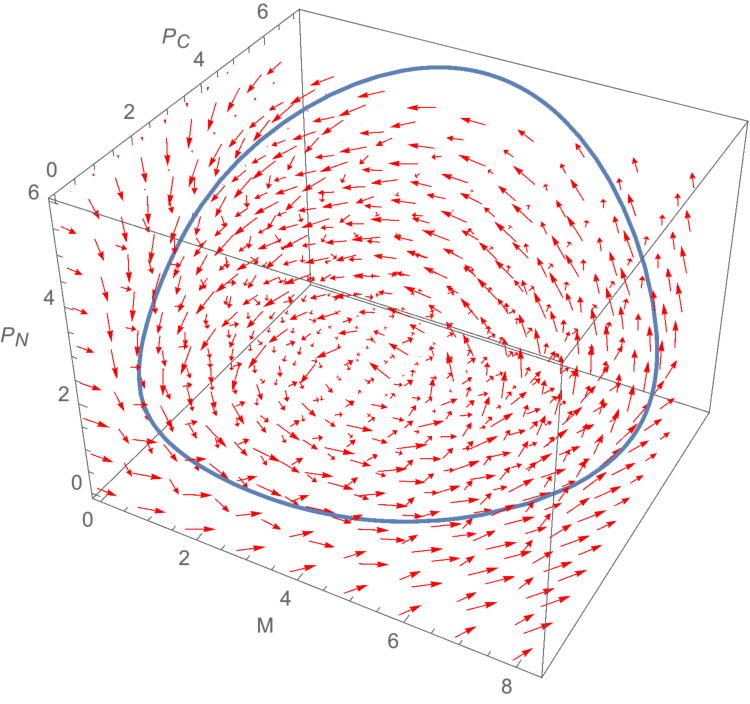
\includegraphics[width=.4\textwidth]{Fig3A.pdf}}
\subfigure[][]{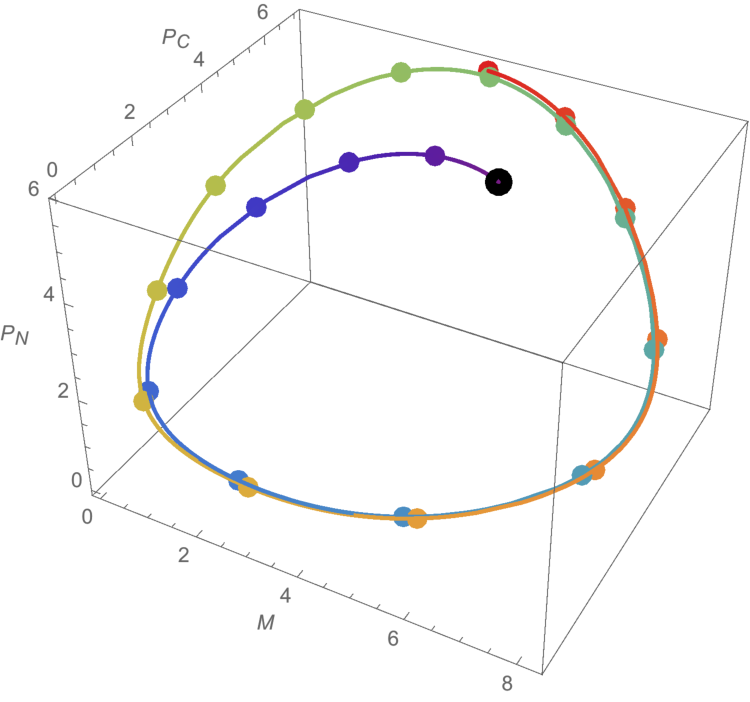
\includegraphics[width=.4\textwidth]{Fig3B.pdf}}
\caption{A. Flow vector field corresponding to the system
  \eqref{eq:Pfeutysystem}. Flow vectors are shown in red, the limit cycle $C$ in
  blue. 
  B. Numerical solution for 48\,h starting from a randomly chosen
  point (black), showing convergence to $C$. Colored dots are placed
  every two hours, with color changing from purple to red with the passage of time. }
\label{fig:LA1}%1
\end{figure}

\begin{figure}[h!]
\centering
\begin{minipage}{.45\linewidth}
\subfigure[][$\nabla\phi(\phi)$]{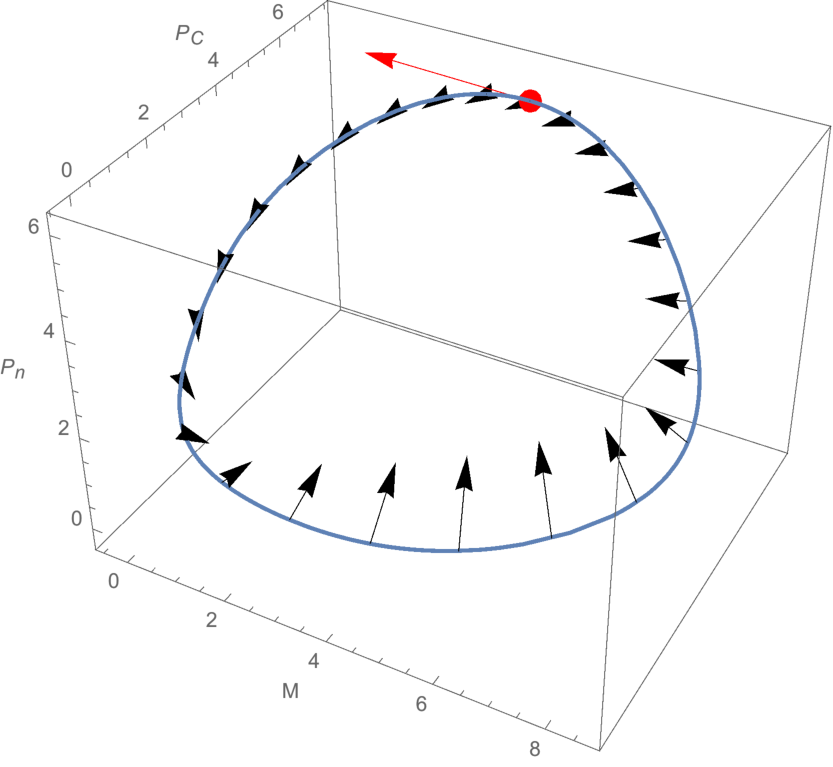
\includegraphics[width=1\textwidth]{Fig4A.pdf}}
\end{minipage}~\begin{minipage}{.32\linewidth}
\subfigure[][$Z(\phi)$]{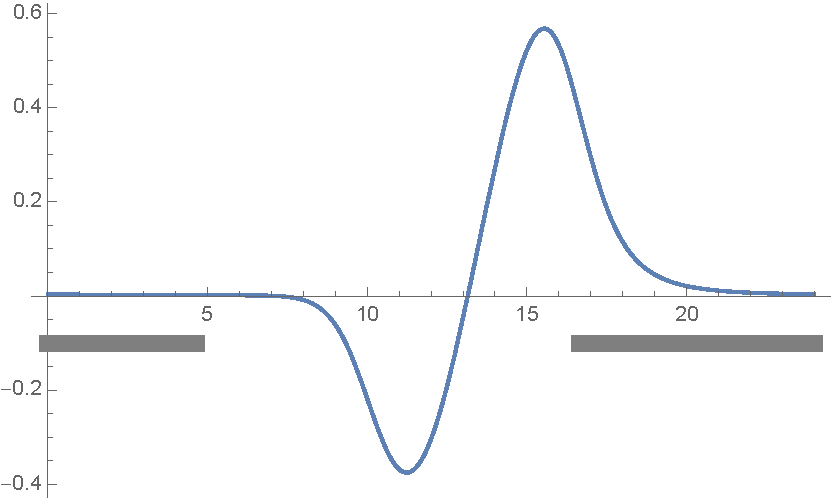
\includegraphics[width=1\textwidth]{Fig4B.pdf}}
\subfigure[][$V(\phi)$]{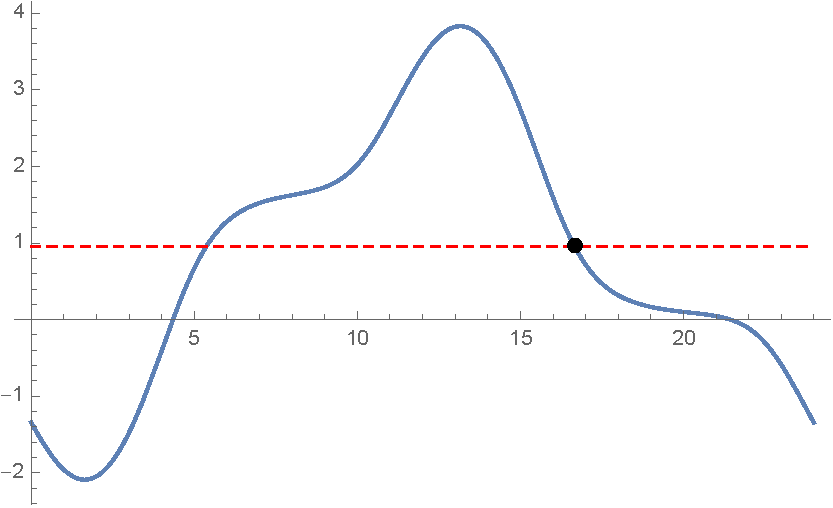
\includegraphics[width=1\textwidth]{Fig4C.pdf}}
\end{minipage}
\caption{
$\nabla\phi$ for the Pfeuty et al (2011) system.
A. In blue is the limit cycle. The red arrow shows the direction of
progress around the cycle. The 24 black arrows show numerically
computed phase gradients at each hour around the cycle. B. The
corresponding IPRC, computed using $\vb{dp}$ being a change of 
$-1$ in parameter ${S}_{M}$. \ The gray bar corresponds to daytime 
$t{\in}[0,\,12]$, based on the resulting PRC in part C. This panel
approximately reproduces the left-hand panel of Pfeuty et al (2011),
\figref{fig:Pfeuty5}A. C. The corresponding PRC with $\epsilon=0.3$, 
$L(t)=2$ if $0{\leq}t{<}12$ and $L(t)=0$ if $12{\leq}t{<}24$. 
With $\gamma =0.96$, there is a stable fixed point 
$\phi^{*}=16.66$, $\chi=-0.799$. This figure approximately reproduces the 
left-hand panel of Pfeuty et al (2011), Figure 2A.
}
\label{fig:LA2}
\end{figure}

\begin{figure}
\centerline{
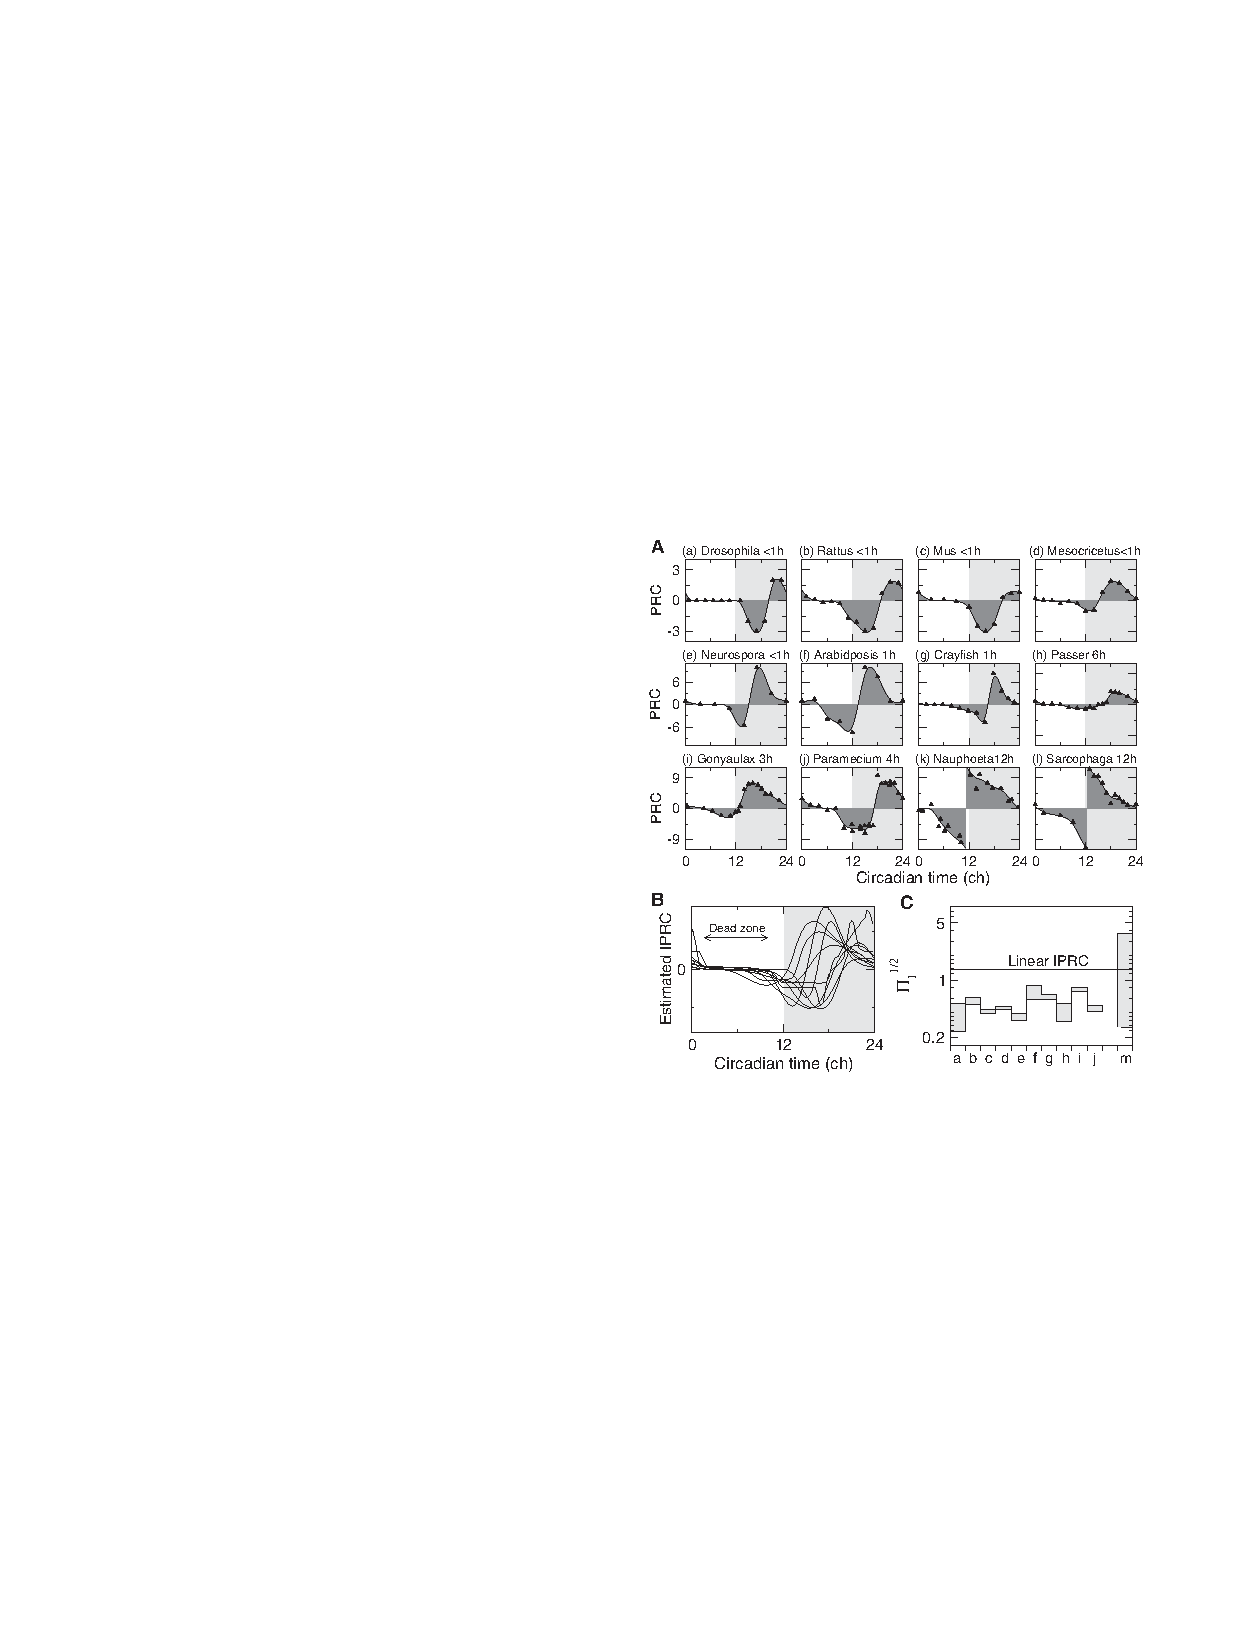
\includegraphics[width=.7\textwidth]{Pfeuty_Fig5.pdf}
}\caption{Experimental IPRCs
show robustness characteristics.
A. Experimentally measured IPRCs collected from the literature. B.
Estimated IPRCs from fitting the data in A. C. a-j: Estimated
robustness measure $\varPi^{1/2}$ computed for experimental IPRCs in
B. m: range of $\varPi^{1/2}$ for all coupling schemes for the
computation al model. Horizontal line: $\varPi^{1/2}$ for an IPRC
that is linearly decreasing during daytime.
This is a copy of Pfeuty et al (2011), Figure 5.
}
\label{fig:Pfeuty5}
\end{figure}

\clearpage








%%% Local Variables: 
%%% mode: latex
%%% TeX-master: "Report_swing_circadian"
%%% End: 
